\chapter{Background}

\section{Paraplegia and Rehabilitation}
Paraplegia is a medical term used to define where a patient loses feeling and/or movement in their lower two limbs. In comparison, quadriplegia (also sometimes known as tetraplegia) is the loss of control in all four limbs. It is important to note that not all feeling/movement needs to be lost in order for someone to be considered paraplegic \cite{IncompleteTraumaticQuadrilegia}. Only 30\% of all paraplegic and quadriplegic patients are considered complete lesions, where there is no sensation and no mobility in the lower limbs \cite{RehabParaplegia}. 

\begin{figure} [h!]
    \centering
    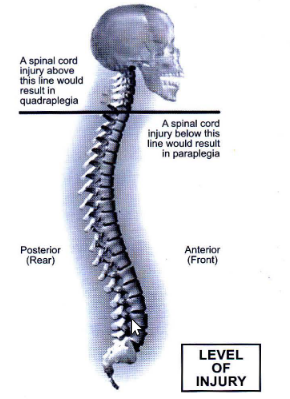
\includegraphics[width=0.5\linewidth]{Figures/Background/ParaQuadInjuryLocs.png}
    \caption{Location of spinal chord injury will determine type of paralysis \cite{RehabParaplegia}}
    \label{fig:ParalysisLocation}
\end{figure}

Paralysis is usually caused by trauma, such as sports injuries, vehicle accidents, or accidental falls, when the spine gets injured (see \autoref{fig:ParalysisLocation}). However, it can also be caused by specific diseases, including multiple sclerosis, amyotrophic lateral sclerosis, and in specific cases cancer \cite{CausesParaplegia}. Common effects of paraplegia include:
 
\begin{itemize}
    \item Loss of mobility, reflexes, and sensation
    \item Muscular weakness and atrophy
    \item Hormonal variations
    \item Gastrointestinal and bowel/bladder problems
    \item Muscle spasms
    \item Reduced cardiorespiratory fitness and increased likelihood of cardiorespiratory issues
\end{itemize}

Rehabilitation can play a key role in reducing these side effects in patients who experience paraplegia. Mainly, physical therapy for paralysis patients focus on three main types of exercises: stretching, strengthening, and aerobic. Additionally, paralysis patients may go through gait training with the assistance of medical devices.

\subsection{Physical Therapy for Paralysis Patients}

\begin{figure}
    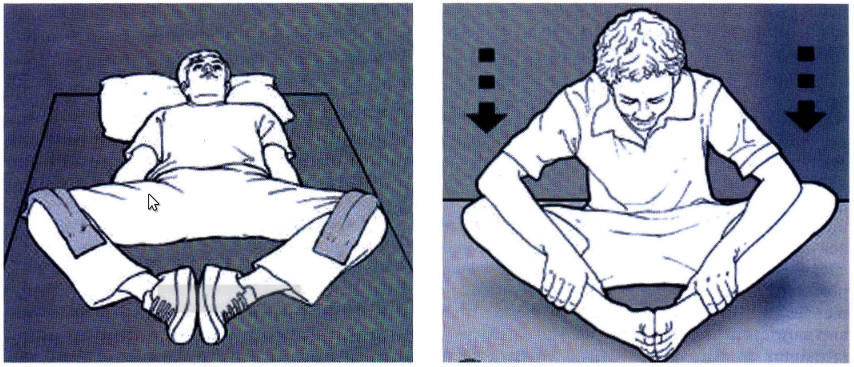
\includegraphics[width=\linewidth]{Figures/Background/BilateralAdductorStretch.png}
    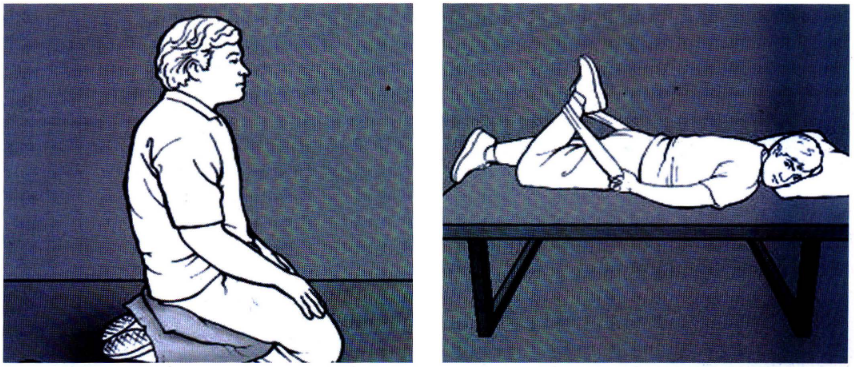
\includegraphics[width=\linewidth]{Figures/Background/QuadricepsStretch.png}
    \caption{Bilateral Adductor Stretches (top) and Quadriceps Stretches (bottom) for paraplegic and quadriplegic patients \cite{RehabParaplegia}}
\end{figure}

Stretching is considered one of the most important exercises \cite{RehabParaplegia}, more-so than any other form of exercise because it can be done often and at home. Carefully designed exercises can improve flexibility, reduce muscle spasms, reduce the chance of injury, and relieve contractures \cite{ParalysisStretchingWeightLoadingPMID} \cite{ParalysisStretchingHarvey} \cite{ParalysisStretchingMichigan}. Some common stretches include bilateral adductor stretches, quadriceps stretches, and hip flexor stretches.

Due to the difficulty of exercise, cardiovascular and cardiorespiratory activities are also very important to maintain health in paralysis patients. Aerobic exercises can increase energy levels, improve lung and heart function, control body weight, and reduce fatigue \cite{RehabParaplegia} \cite{AerobicCapacityParaplegia}. A study showed that patients who suffer from neuromuscular deficiencies such as paraplegia suffered decreasing VO\textsubscript{2} max compared to control subjects with no issues \cite{AerobicCapacityParaplegia}. VO\textsubscript{2} max a common metric that measures the maximum rate of oxygen utilization during heavy exercise. Combination of the upper body and lower body in paraplegic patients can strengthen the paralyzed limbs while also activating healthy limbs.

Improving strength in muscles may actually partially reverse the loss of mobility in partially paralyzed patients, while also improving muscle tone \cite{AerobicCapacityParaplegia} and preventing bone atrophy \cite{ParalysisStretchingWeightLoadingPMID}. This type of exercise can be split into two major regions: training of affected limbs and muscles, and the training of non-affected regions. Affected limbs can benefit from an increase in mobility and definition, and can generally reduce the likelihood of muscular atrophy. Additionally, strong hip and leg muscles in partially paraplegic patients can help in gait training and increase the possibility of usage in life. On the other side, increasing or maintaining strength in unaffected regions can help with quality of life improvement. Often, paraplegic patients may elect to use crutches or canes as an assisted mobility device in the real world. Increasing arm/shoulder strength and endurance will also increase capability for patients to use some of these assisted devices. Finally, back and abdomen muscles are very important to strengthen to maintain posture and improve gait performance \cite{TrunkMuscleLoadingParaplegia}. 

\subsection{Gait Training}

\subsection{Use of Assistive Devices}

% Don't forget to talk about skin rubbing in assistive devices

\section{Robotics for Paraplegia}


\section{Previous work on Exoskeleton Orthosis}
Exoskeletons are an interesting application to help those with walking disabilities rehabilitate and exercise their muscles.

\subsection{Rewalk}

\subsection{Esko}

\subsection{Indigo}

\section{WPI LARRE Exoskeleton}
% LARRE Stands for Legged Articulated Robotic Rehabilitation Exoskeleton 

\section{Research in the Human Knee Joint}
